\documentclass[10pt,twocolumn,letterpaper]{article}
\usepackage[T1]{fontenc}
\usepackage{lmodern}
\usepackage{microtype}
\usepackage[margin=0.75in, top=0.85in, bottom=0.85in]{geometry}
\usepackage{amsmath,amssymb,amsfonts}
\usepackage{booktabs}
\usepackage{graphicx}
\usepackage{xcolor}
\usepackage{caption}
\usepackage{fancyhdr}
\usepackage{abstract}
\usepackage{titlesec}
\usepackage{enumitem}
\usepackage{hyperref} % load last

\definecolor{mospNavy}{HTML}{0F172A}
\definecolor{mospBlue}{HTML}{0284C7}
\definecolor{mospEmerald}{HTML}{059669}
\definecolor{mospRose}{HTML}{E11D48}
\definecolor{mospGray}{HTML}{475569}

% Placeholder for values that must come from model output. Renders in red so nothing ships unfilled.
\newcommand{\TBD}[1]{\textcolor{mospRose}{\textbf{[#1]}}}

\hypersetup{colorlinks=true, linkcolor=mospBlue, citecolor=mospEmerald, urlcolor=mospBlue}
\pagestyle{fancy}
\fancyhf{}
\fancyhead[L]{\footnotesize \textbf{\textcolor{mospGray}{THE MINISTRY OF SILLY PLOTS}} $\vert$ \texttt{sillyplots.com}}
\fancyhead[R]{\footnotesize \textit{\textcolor{mospGray}{Working Paper No. 2026-11: Broadcast Clich\'{e} Econometrics}}}
\fancyfoot[C]{\footnotesize \thepage}
\renewcommand{\headrulewidth}{0.4pt}

\titleformat{\section}{\large\bfseries\color{mospNavy}}{\thesection.}{0.5em}{}
\titleformat{\subsection}{\normalsize\bfseries\color{mospBlue}}{\thesubsection.}{0.5em}{}

\title{\vspace{-1.5em}\textbf{\LARGE Is It Really Tough to Beat a Team Twice?\\ An Econometric Autopsy of Broadcast Booth Folklore}\vspace{0.4em}\\
\large \textit{Or: Why Winning Football Games Is Surprisingly Positively Correlated With Winning Subsequent Football Games}}

\author{
    \textbf{Office of Gridiron Narratives \& Spurious Folklore}\\
    The Ministry of Silly Plots (\texttt{sillyplots.com})\\
    \texttt{fellows@sillyplots.com}
}
\date{November 2026}

\begin{document}
\twocolumn[
  \begin{@twocolumnfalse}
    \maketitle
    \vspace{-1em}
    \begin{abstract}
      \noindent Every January, normally functional adults wearing quarter-zips on national television look directly into a camera and intone one of civilization's most cherished falsehoods: \textit{``You know, Jim, it is almost impossible to beat a team three times in one season.''} This paper investigates the ``Tough to Beat a Team Twice (or Thrice)'' hypothesis across $1{,}299$ same-season NFL rematch games. Following our previous inquiry into the \textit{Home Brew Advantage}---which forecast a Seahawks victory in Super Bowl LX on the grounds that Levi's Stadium is the second most Starbucks-dominant venue in the league ($G_{\text{net}} = -5.80$)---we once again deploy serious econometric machinery against a defenseless sports narrative. Teams that won the prior meeting win the rematch \textbf{57.9\%} of the time overall. Controlling for roster quality via a Leave-One-Opponent-Out Expected Points Added ($\text{LOOO-EPA}$) logistic model and for venue alternation, no rematch penalty is found: the estimate is slightly positive and statistically indistinguishable from zero ($\hat\gamma = +0.12$, $p = 0.07$). It turns out that being better at football in October remains a remarkably durable asset in December.
      \vspace{0.8em}

      \noindent \textbf{Keywords:} NFL Analytics, Broadcast Clich\'{e}s, Conditional Probability Malpractice, Leave-One-Out EPA, Regression to the Mean, Quarter-Zip Epistemology.
      \vspace{1.2em}
      \hrule
      \vspace{1.5em}
    \end{abstract}
  \end{@twocolumnfalse}
]

%==========================================================
\section{Introduction: The Quarter-Zip Fallacy}
%==========================================================
In our prior working paper (\textit{Home Brew Advantage}, Feb.\ 2026), this Ministry introduced the Interference-Adjusted Exponential Decay Model of regional coffee gravity and identified Levi's Stadium as a Starbucks stronghold ($G_{\text{net}} = -5.80$), second only to Lumen Field itself. We forecast that a Dunkin'-dependent Patriots offense would struggle there. The Seahawks won.

Emboldened, we turn to a far more insidious piece of folk wisdom that continues to pollute NFL broadcasts every Sunday: the belief that \textbf{defeating an NFL opponent once makes it inherently harder to defeat them a second (or third) time in the same season.}

The appeal of the clich\'{e} is easy to understand. Every broadcaster remembers the 2007 Giants. Nobody remembers the many sweeping teams that simply won again, because ``better team wins again'' does not fill a pregame segment.

We propose the following hypotheses:
\begin{itemize}[leftmargin=1.2em, itemsep=2pt]
  \item \textbf{H1 (The Booth Hypothesis).} Holding team quality and venue constant, winning the prior meeting \textit{reduces} the probability of winning the rematch ($\gamma < 0$).
  \item \textbf{H2 (The Familiarity Hypothesis).} Rematches are closer than first meetings, as opponents neutralize each other's tendencies.
  \item \textbf{H3 (Null Hypothesis).} Any apparent rematch effect is an artifact of team quality, home-field alternation, and regression to the mean.
\end{itemize}

%==========================================================
\section{Data}
%==========================================================
Our sample comprises three families of same-season rematches:
\begin{itemize}[leftmargin=1.2em, itemsep=2pt]
  \item \textbf{Regular-season divisional series}, 2002--2025 ($n = 1{,}145$ Game~2s). Twenty-four seasons of 48 divisional pairs yield $1{,}152$ series; we exclude 6 in which Game~1 was tied (no prior winner) and 1 in which Game~2 was tied.
  \item \textbf{Non-divisional playoff rematches}, 2002--2025, in which a team met a regular-season opponent again in the postseason ($n = 129$).
  \item \textbf{Three-game sweep attempts}, 1970--2025, in which a team swept a divisional rival $2\text{--}0$ and met it a third time in the playoffs ($n = 25$; the earliest occurs in 1982, the latest in 2022).
\end{itemize}
Because post-2002 sweep attempts also appear in the divisional sample as Game~2 observations, we refer to $1{,}299$ rematch \textit{games} rather than independent series.

Game results and play-by-play data for 1999--2025 were sourced from nflverse. Results for 1970--1998 come from FiveThirtyEight's public NFL game file. Because nflverse EPA begins in 1999, the 12 sweep attempts from 1970--1998 have no LOOO-EPA and are excluded from the regression in Section~4.

%==========================================================
\section{The Naive Data: A Massacre of Conventional Wisdom}
%==========================================================
Table~\ref{tab:naive} reports raw rematch records. Across all $1{,}299$ rematch games, the winner of the prior meeting won \textbf{57.9\%} of the time: $+7.9$ percentage points ($+15.8\%$ relative) above a coin flip.

\begin{table}[h]
\centering
\small
\caption{Prior-winner record in rematches. 95\% Wilson intervals.}
\label{tab:naive}
\begin{tabular}{@{}lccc@{}}
\toprule
\textbf{Rematch type} & \textbf{W--L} & \textbf{Win\%} & \textbf{95\% CI} \\
\midrule
Divisional (Game 2)     & 662--483 & 57.8 & 54.9--60.6 \\
Playoff, non-div.       & 74--55   & 57.4 & 48.7--65.6 \\
Three-game sweep        & 16--9    & 64.0 & 44.5--79.8 \\
\midrule
\textbf{All rematches}  & 752--547 & \textbf{57.9} & 55.2--60.5 \\
\bottomrule
\end{tabular}
\end{table}

The three-game sweep figure, so beloved of January pregame shows, rests on 25 observations. Its confidence interval comfortably contains both the overall rematch rate and, for that matter, a coin flip. We report it because the booth insists on discussing it, not because it tells us much.

Of course, a 57.9\% rematch rate does not by itself refute the booth. Good teams win Game~1, and good teams also win Game~2. To isolate the effect of \textit{having beaten this particular opponent}, we must hold team quality constant.

%==========================================================
\section{Methodology: The Econometric Autopsy}
%==========================================================
\subsection{Leave-One-Opponent-Out EPA}
A team's season-long EPA is contaminated by the very games we are trying to explain. We therefore compute each team's net EPA per play excluding all games against the rematch opponent:
\begin{equation}
\text{LOOO-EPA}_{i,j} = \overline{\text{EPA}}^{\,\text{off}}_{i,\,-j} - \overline{\text{EPA}}^{\,\text{def}}_{i,\,-j}
\end{equation}
where $-j$ denotes all of team $i$'s regular-season games except those against opponent $j$.

\subsection{Model Specification}
For each rematch game $g$ between prior winner $i$ and prior loser $j$, we estimate:
\begin{equation}
\begin{split}
\text{logit}\,\Pr(W_{g} = 1) = \alpha &+ \beta\,\Delta\text{EPA}_{g} + \delta\,\text{Home}_{g} \\
&+ \gamma\,\text{Rematch}_{g} + \varepsilon_{g}
\end{split}
\end{equation}
where $W_g$ indicates a team win, $\Delta\text{EPA}_g = \text{LOOO-EPA}_{i,j} - \text{LOOO-EPA}_{j,i}$, $\text{Home}_g$ is a home-field indicator, and $\text{Rematch}_g$ indicates that the team won the prior meeting. Each rematch enters the model twice, once per team, with $\text{Rematch}_g = 1$ for the prior winner and $0$ for the prior loser. Because the two rows mirror each other, $\alpha$ is pinned at zero, and we estimate the model on one row per game from the prior winner's perspective, with $\text{Home}_g$ coded $+1$ (home), $-1$ (away) or $0$ (neutral site). The comparison is therefore between the prior winner's actual rematch result and the result predicted by quality and venue alone. Under H1, $\gamma < 0$. A companion OLS model with the prior winner's point margin as the outcome asks the same question of the scoreboard. H2 is tested separately (Section~5.2).

\begin{figure*}[t]
\centering
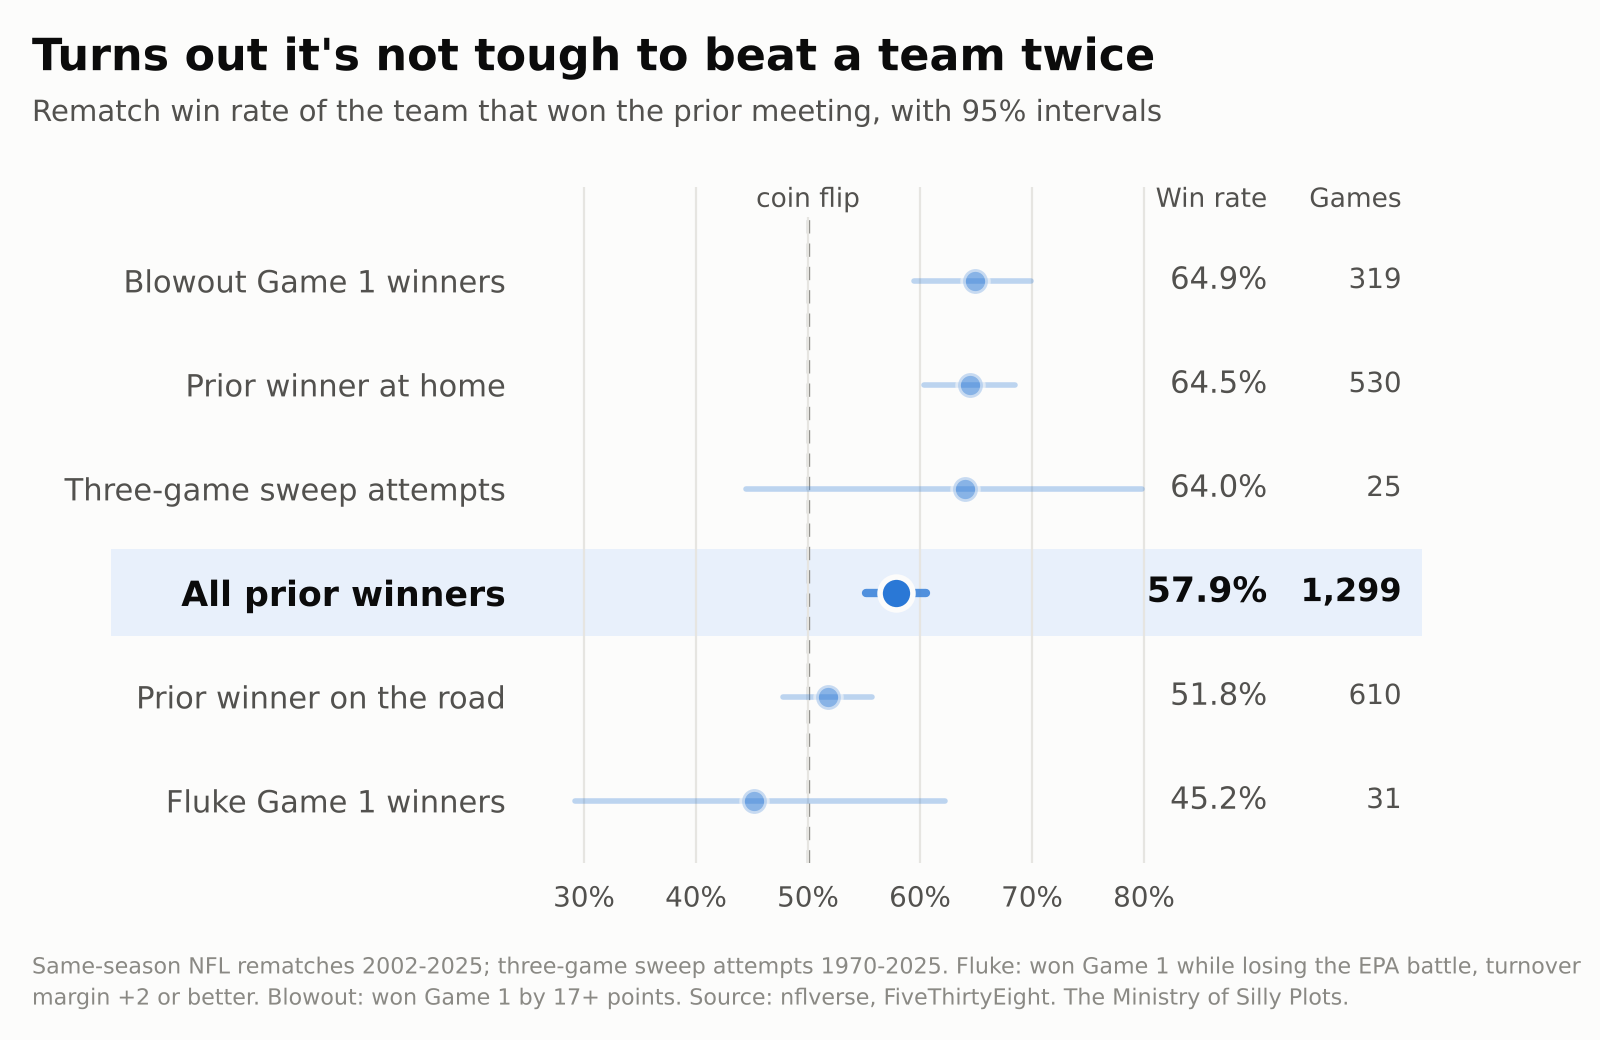
\includegraphics[width=0.82\textwidth]{../assets/rematch_win_rates.png}
\caption{Rematch win rate of the prior-meeting winner, by situation, with 95\% Wilson intervals.}
\label{fig:rates}
\end{figure*}
\subsection{Control Variables: The Venue Alternation Problem}
Divisional series alternate venues. Because home teams win more often, Game~1 winners are disproportionately teams that were \textit{at home} in Game~1, and are therefore disproportionately \textit{on the road} in Game~2. In our divisional sample, 53.3\% of Game~1 winners played Game~2 away from home. Those playing Game~2 at home won 64.5\% of rematches; those on the road won 51.8\%.

The imbalance itself is mild. Had Game~1 winners been split evenly between home and road rematches, the naive divisional rate would rise by only $0.35$ points, to 58.2\%. The venue effect within each game is not mild: a prior winner on the road is barely better than a coin flip. These road rematches supply the booth with its anecdotes. The booth has, in effect, rediscovered home-field advantage and mistaken it for a curse.

%==========================================================
\section{Results}
%==========================================================
\subsection{The Rematch Penalty (Not Found)}

\begin{table}[h]
\centering
\small
\caption{Rematch outcome models. Standard errors in parentheses.}
\label{tab:reg}
\begin{tabular}{@{}lcc@{}}
\toprule
 & \textbf{(1) Logit} & \textbf{(2) OLS} \\
 & Win & Margin \\
\midrule
$\Delta$LOOO-EPA ($\beta$) & $4.74$ & $37.93$ \\
                           & $(0.45)$ & $(2.57)$ \\
Home ($\delta$)            & $0.27$ & $2.38$ \\
                           & $(0.06)$ & $(0.37)$ \\
Rematch ($\gamma$)         & $0.12$ & $0.84$ \\
                           & $(0.06)$ & $(0.40)$ \\
\midrule
$N$                        & $1{,}287$ & $1{,}287$ \\
Pseudo-$R^2$ / $R^2$       & $0.086$ & $0.174$ \\
\bottomrule
\multicolumn{3}{@{}p{0.92\columnwidth}@{}}{\footnotesize Rematch games 2002--2025 and sweep attempts 1999--2025 with play-by-play data. $\gamma$ is the prior-winner intercept (Section~4.2).}
\end{tabular}
\end{table}

The estimated rematch penalty is $\hat\gamma = +0.12$ ($p = 0.07$; 95\% CI $-0.01$ to $+0.24$ on the log-odds scale). It has the wrong sign. Evaluated at the sample mean, it corresponds to a change in rematch win probability of $+2.8$ percentage points, with a 95\% interval of $-0.2$ to $+5.8$. The margin model agrees: prior winners outscore their predicted margin by $0.84$ points ($p = 0.03$).

The most likely explanation for the positive estimate is mundane. LOOO-EPA deliberately discards the head-to-head games, so the result of the prior meeting probably retains some information about how the two teams match up. Having beaten a team is, if anything, mild evidence that one can beat them again.

We note, in the interest of scholarly integrity, that the interval does not quite exclude zero. It does exclude any penalty larger than a fraction of a point, and it rules out the booth's preferred magnitude, which is ``almost impossible.''

\noindent\textbf{Conclusion: H1 is Not Supported.}

\subsection{Familiarity (Not Found)}
Across $2{,}304$ divisional games, regressing the absolute point margin on a Game~2 indicator and the season-long EPA gap between the two teams, rematch margins are $0.60$ points \textit{wider} than first-meeting margins (95\% CI $-0.12$ to $+1.32$; $p = 0.10$; standard errors clustered by series), against a typical Game~1 margin of $11.2$ points. Familiarity does not visibly compress anything.

\noindent\textbf{Conclusion: H2 is Not Supported.}

\subsection{Fluke Winners and Regression to the Mean}
Stratifying Game~1 winners by how they won exposes the mechanism behind the folklore (Table~\ref{tab:strata}).

\begin{table}[h]
\centering
\small
\caption{Rematch win rate by Game 1 profile.}
\label{tab:strata}
\begin{tabular}{@{}lccc@{}}
\toprule
\textbf{Game 1 profile} & \textbf{$n$} & \textbf{Win\%} & \textbf{95\% CI} \\
\midrule
Fluke winner$^{a}$   & 31 & 45.2 & 29.2--62.2 \\
Blowout winner$^{b}$ & 319 & 64.9 & 59.5--69.9 \\
\bottomrule
\multicolumn{4}{@{}p{0.92\columnwidth}@{}}{\footnotesize $^{a}$Won Game 1 while losing the EPA battle, with turnover margin $\geq +2$. $^{b}$Won Game 1 by 17 or more points. Prior meetings 1999--2025 with play-by-play data.}
\end{tabular}
\end{table}

Teams that won Game~1 by winning the turnover lottery go on to lose the rematch more often than not (14--17). The fluke sample is small and its interval wide, but the gap to blowout winners is statistically distinguishable ($p = 0.03$, two-proportion test).

The gap is explained by quality. Fluke winners held essentially no LOOO-EPA edge over their opponents (mean $\Delta\text{EPA} = -0.007$, against $+0.102$ for blowout winners). Adding fluke and blowout indicators to the logit model leaves both indistinguishable from zero ($p = 0.80$ and $p = 0.34$). Fluke winners lose rematches at exactly the rate their quality predicts. This is not because beating a team twice is hard. It is because they were never the better team, and the bounces stopped bouncing. The booth, observing these teams, has mistaken regression to the mean for a law of nature.

\noindent\textbf{Conclusion: H3 is Supported.}

%==========================================================
\section{Conclusion}
%==========================================================
Figure~\ref{fig:rates} summarizes the evidence. Rematch outcomes track quality and venue; the prior meeting adds nothing the booth would recognize as a curse. Based on $1{,}299$ rematch games and econometric controls for quality and venue, the Ministry of Silly Plots officially classifies \textit{``It's tough to beat a team twice''} as \textbf{Grade-A Broadcast Mythology}. It is tough to beat a \textit{better} team twice. It is tough to beat a team twice \textit{on the road}. It is tough to win a second turnover lottery. It is not especially tough to beat a team twice.

%==========================================================
\section{Code Artifacts \& Reproducibility}
%==========================================================
All analysis code is available in the project repository at:\\
\url{https://github.com/sillyplots/mosp/blob/main/posts/rematch/README.md}

\end{document}
